\subsection{Client - Java}
\label{sec:Javaclient}

Der hier beschriebene Javaclient ist ein möglicher Teilnehmer, der sich mit den Kommunikationsserver verbinden und ein Spiel austragen kann.
Sein Design orientiert sich am Model-View-Controller (MVC) Prinzip, wobei das Spielbrettmodell auf Grund seines geringen Umfangs im Controller eingebettet wurde.

Eine Übersicht des Entwurfs wird in Abbildung \ref{fig:Javaclientklassendiagramm} dargestellt.
Die beiden Klassen \texttt{CBattleShipGUI} und \texttt{CPlayingFieldPanel} bilden den \emph{View} Bestandteil des MVC Prinzips ab.

\begin{figure}[H]
  \centering
  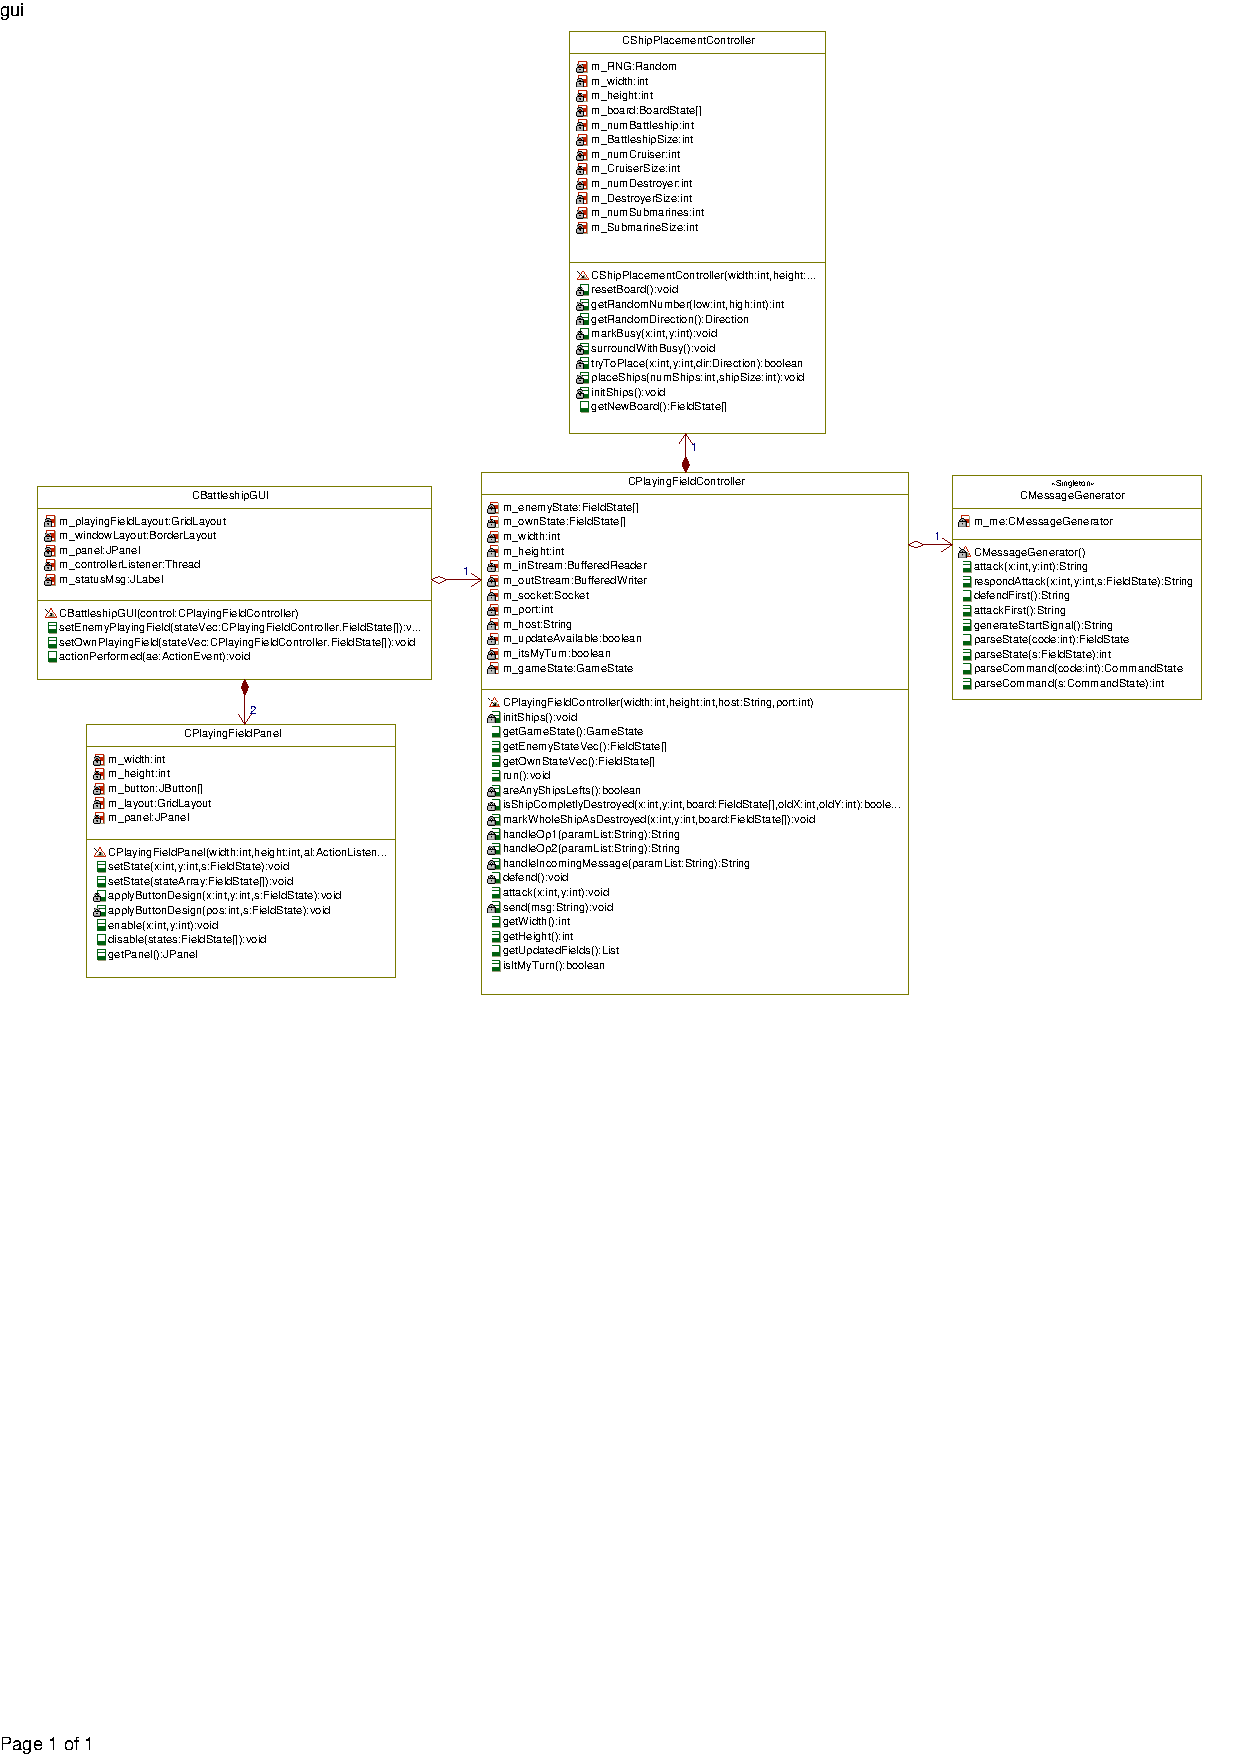
\includegraphics[trim=5mm 125mm 5mm 4mm,clip,width=0.9\textwidth]{images/CJavaClient.pdf}
  \caption{Klassendiagramm des Java Clients}
  \label{fig:Javaclientklassendiagramm}
\end{figure}

\subsubsection{View}

Das eigene, sowie das gegnerische Spielfeld werden durch jeweils eine Instanz der Klasse \texttt{CPlayingFieldPanel} visualisiert, wie es in Abbildung \ref{fig:Spielfeldpanel} zu sehen ist.
Dieses besteht primär aus einem gitterförmigen Spielfeld, dessen Spielfeldzustände durch Farben codiert sind.
Das hier gezeigte Spielfeld stellt das eigene Wissen des gegnerischen Spielfelds dar.
Die grauen Felder symbolisieren noch unbekanntest Terrain.
Blau bedeutet, dass bei einem vorangegangenen Angriff ein Feld mit Wasser getroffen wurde.
Rot symbolisiert ein getroffenes, jedoch noch nicht versenktes Schiff.
Versenkte Schiffsfelder sind schwarz gehalten.

\begin{figure}[H]
  \centering
  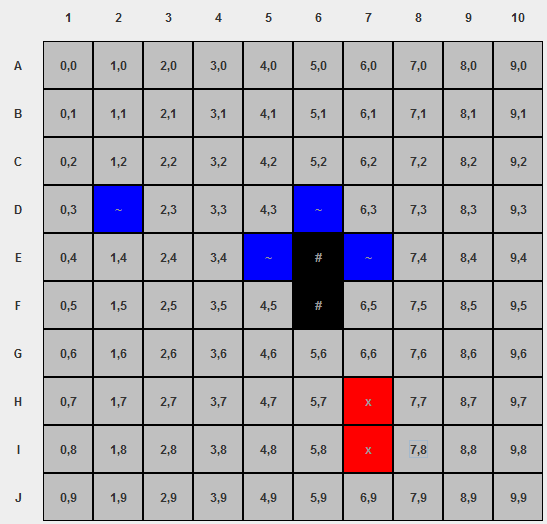
\includegraphics[width=0.5\textwidth]{images/JavaPlayingFieldPanel.png}
  \caption{Gegnerisches Spielfeld mit einem zerstörten (schwarz) und einem beschädigten Schiff (rot)}
  \label{fig:Spielfeldpanel}
\end{figure}

Die visuelle Codierung des eigenen Spielfeldes wird analog zum gegnerischen Feld vorgenommen.
Hier sind standardmäßig alle Felder aufgedeckt und wie in Abbildung \ref{fig:EigenesSpielfeldpanel} zu sehen ist, blau eingefärbt.
Die eigenen Schiffe sind ebenfalls sichtbar und mit dunkelgrauer Farbe hervorgehoben.
Angriffe des Gegners, die das Wasser getroffen haben, sind hellblau dargestellt.
Analog zum gegnerischen Spielfeld sind Treffer rot und versenkte Schiffe schwarz eingefärbt.

\begin{figure}[H]
  \centering
  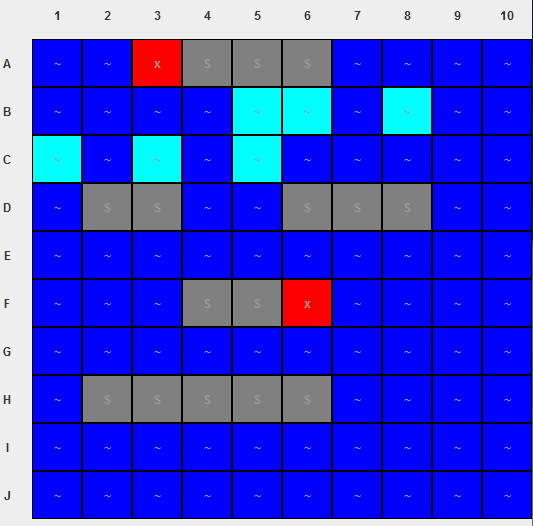
\includegraphics[width=0.5\textwidth]{images/JavaOwnPlayingFieldPanel.png}
  \caption{Eigenes Spielfeld mit beschädigten Schiffen (rot) und misglückten Angriffen des Gegners (hellblau)}
  \label{fig:EigenesSpielfeldpanel}
\end{figure}

Die GUI-Oberfläche besteht primär aus zwei Instanzen der Klasse \texttt{CPlayingFieldPanel}, die jeweils das eigene und gegnerische Spielfeld abbilden.
Wie in Abbildung \ref{fig:GUI} zu erkennen ist befindet sich über jedem Spielfeld eine Überschrift, die die Zugehörigkeit signalisiert.
Des Weiteren befindet sich in der unteren linken Ecke ein Statusfeld, das angibt, wer den nächsten Spielzug auszuführen hat bzw. ob man das Spiel verloren bzw. gewonnen hat.
Sollte der Gegner am Zug sein, so wird gleichzeitig das gesamte Spielfeld deaktiviert, sodass keine Buttonaktionen ausgeführt werden können.

\begin{figure}[H]
  \centering
  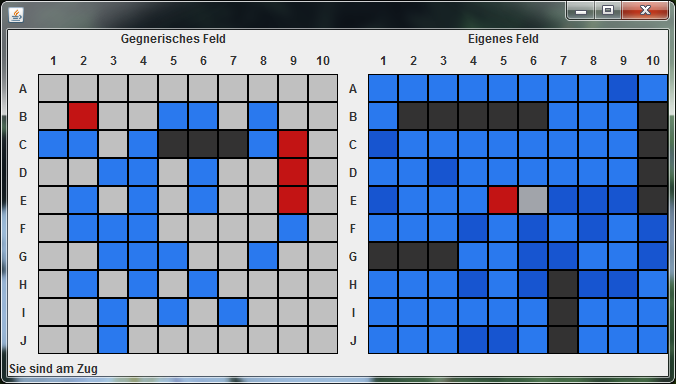
\includegraphics[width=0.9\textwidth]{images/JavaClientGUI.png}
  \caption{Gesamte Benutzeroberfläche}
  \label{fig:GUI}
\end{figure}

\subsubsection{Controller / Model}

Die Klasse \texttt{CPlayingFieldController} ist das zentrale Element der Spielsteuerung und wertet die eingehenden Nachrichten und Signale aus.
Des Weiteren beinhaltet diese Klasse auch die Model-Komponente in Form zweier Arrays, die die Spielfelder repräsentieren.
Der Abruf dieser Daten orientiert sich am Observer Entwurfsmuster.
Jede Änderung an diesen Arrays wird mittels der javaeigenen Methode \texttt{notifyAllObservers()} den Beobachtern mitgeteilt.

Der Controller-Anteil wird durch die Erzeugung eines Threads realisiert, der eingehende Netzwerknachrichten annimmt und auswertet.
Zur Generierung ausgehender Nachrichten, die einen Angriff signalisieren, dient die Methode \texttt{attack(int x, int y)} und wird durch die Interaktion mit der GUI aufgerufen.
Sowohl der Thread, als auch die GUI-Interaktion blockieren sich auf Basis von Monitoren gegenseitig, die mit dem Schlüsselwort \texttt{synchronized} signalisiert werden.
Mittels dieser Technik wird verhindert, dass die beiden Zustände \emph{ATTACK} und \emph{DEFENCE} unsachgemäß eingenommen werden.

Eingehende Angriffe werden durch den Vergleich mit dem eigenen Spielfeld behandelt und das Ergebnis per Nachricht bekannt gegeben.
Gleichzeitig wird der Status des eigenen Spielfeldes an der entsprechenden Stelle aktualisiert.
Im Fall von Wasser wird an dieser Position der Status Verfehlt gesetzt.
Bei einem Schiff wird der Status auf Getroffen geändert.
Gleichzeitig wird eine Routine gestartet, die überprüft, ob das das ganze Schiff versenkt wurde.
Ist dem so, so wird wiederum eine Routine gestartet, die überprüft, ob alle Schiffe versenkt wurden.
Die entsprechenden Ergebnisse werden per Netzwerkantwort übermittelt.
Sind keine eigenen Schiffe mehr vorhanden, oder ging die Nachricht ein, dass der Gegner über keine Schiffe mehr verfügt, so wird der Spielstatus auf verloren, bzw. gewonnen gesetzt.

Die Generierung der prologkompatiblen Nachrichten wird in der Klasse \texttt{CMessageGenerator} vorgenommen.
Diese bietet für jede Aktion und Reaktion passende Methoden an und liefert den gewünschten zu übertragenen Text.
Diese Klasse ist ebenfalls für die Dekodierung der Opcodes und Ergebnisse in interne Enumerationen zuständig.

In der Initialisierungphase ruft der Controller die Klasse \texttt{CShipPlacementController} auf.
Diese Klasse ist für die regelkonforme Platzierung der Schiffe auf dem Spielbrett zuständig.
Der Vorgang zum Platzieren eines Schiffes ist dabei von seinem Typ und somit seiner Größe unabhängig und kann wie folgt beschrieben werden:
\begin{enumerate}
	\item Generiere zufällig die $x/y$ Position, sowie die Orientierung, in der das Schiff platziert werden soll.
	\item Prüfe ob diese Position belegt ist, oder ob sich in der direkten 8er Nachbarschaft ein Schiff befindet. 
	Es gilt ebenfalls die Spielfeldgrenzen zu berücksichtigen.
	\item Wiederhole den vorherigen Schritt rekursiv an der nächsten Position in angegebener Orientierung. 
	Die Schiffsgröße wird mit jedem Rekursionsschritt um 1 verringert, sodass aus dieser Angabe die Abbruchbedingung erzeugt werden kann.
	\item Wurde in keinem Feld rekursiv eine Behinderung festgestellt, werden die Felder mit der Schiffskennung versehen.
\end{enumerate}
Diese vier Verarbeitungsschritte werden für jedes zu platzierende Schiff aufgerufen.
Jedoch ist nicht gewährleistet, dass eine zufällig generierte Position auch frei ist.
Deshalb steht pro Schiffstyp ein maximales Kontingent an Versuchen zur Verfügung, das sich nach jedem erfolgreich platzierten Schiff wieder füllt.
Sollte das Kontingent für einen Schiffstypen aufgebraucht worden sein, so wird das Gesamtkontingent für das gesamte Spielbrett reduziert und das gesamte Spielbrett wird zurückgesetzt.
Sollte auch dieses Kontingent aufgebraucht worden sein, wird eine Fehlermeldung per Exception ausgegeben.